% 1. ročník, hodina 65. Podklad: autorova učebnice Lineární funkce.tex;
% návaznost na vlastní přípravy 63 a 64. Metodická inspirace:
% Realisticky.cz 020109–020111 (grafy lineárních a konstantních funkcí).
% Všechny příklady a grafy jsou pro tento dokument nově zpracovány.
\documentclass[11pt,a4paper]{article}
\input{../../sablony/pripravy/priprava.sty}
\usepackage{tikz}
\usetikzlibrary{arrows.meta}
\nastavPripravu{1. ročník}{Funkce}{65}{Grafy lineárních a konstantních funkcí}
\begin{document}
\poznamka{Na 45 minut: návaznost a opakování 4 min; konstantní funkce 8 min;
průsečíky s osami 10 min; omezený definiční obor 10 min; samostatná práce 9 min;
kontrola a shrnutí 4 min. Druhý řešený příklad a další otázky lze přesunout mezi domácí úlohy.
Neopakuj celý pracovní list z hodiny 64: dnes jde o interpretaci grafu, nikoli o opakované rýsování přímek.}

\blok{Navazujeme na lineární funkci}
V hodinách 63--64 jsme pracovali s předpisem $f(x)=ax+b$, sestrojovali grafy a měnili
parametry $a$ a $b$. Připomeňme si, že při $a=0$ se funkční hodnota při změně
argumentu vůbec nemění. Takový zvláštní případ si dnes přesně pojmenujeme.
Zároveň u grafu vyhledáme body na souřadnicových osách a budeme hlídat
\emph{skutečně zadaný definiční obor}.

\begin{definiceBox}
\textbf{Konstantní funkce} na neprázdném definičním oboru $D(f)$ je funkce, pro kterou existuje
$c\in\mathbb R$ tak, že
\[
  f(x)=c\qquad\text{pro každé }x\in D(f).
\]
Je-li $D(f)=\mathbb R$, jejím grafem je vodorovná přímka $y=c$.
Je zvláštním případem lineární funkce $f(x)=ax+b$ pro $a=0$ a $b=c$.
\end{definiceBox}

\begin{prikladReseniBox}[title={Příklad 1: konstantní funkce na různých oborech}]
Porovnejte grafy funkcí $g(x)=2$ na $\mathbb R$ a $h(x)=2$ na
$D(h)=\{-2,0,3\}$. Určete definiční obor a obor hodnot obou funkcí.
\tcblower
Obě funkce nabývají jediné hodnoty $2$, takže $H(g)=H(h)=\{2\}$.
První graf je celá vodorovná přímka $y=2$ a $D(g)=\mathbb R$.
Druhý graf tvoří \emph{jen tři body} $[-2;2]$, $[0;2]$ a $[3;2]$;
$D(h)=\{-2,0,3\}$. Body nespojujeme.
\end{prikladReseniBox}

\begin{center}
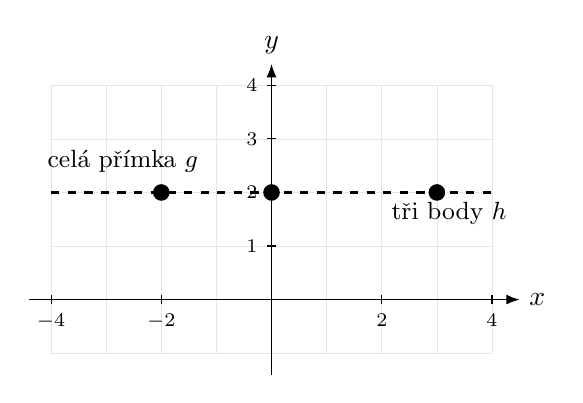
\begin{tikzpicture}[x=.70cm,y=.68cm,>=Latex]
  \draw[step=1,gray!20,very thin] (-4,-1) grid (4,4);
  \draw[->] (-4.4,0)--(4.5,0) node[right] {$x$};
  \draw[->] (0,-1.4)--(0,4.4) node[above] {$y$};
  \foreach \x in {-4,-2,2,4}{\draw (\x,.08)--(\x,-.08) node[below,font=\scriptsize] {$\x$};}
  \foreach \y in {1,2,3,4}{\draw (.08,\y)--(-.08,\y) node[left,font=\scriptsize] {$\y$};}
  \draw[thick,dashed] (-4,2)--(4,2);
  \foreach \x in {-2,0,3}{\fill (\x,2) circle (3pt);}
  \node[font=\small,above] at (-2.7,2.2) {celá přímka $g$};
  \node[font=\small,below right] at (2,2) {tři body $h$};
\end{tikzpicture}
\end{center}
\poznamka{Čárkovaná přímka představuje graf $g$. Vyplněné body samy představují graf $h$.
Při výkladu odděl, zda žák má spojovat \emph{všechny} hodnoty $x$, nebo jen vypsané argumenty.}

\blok{Průsečíky grafu se souřadnicovými osami}
Průsečík s osou $y$ má první souřadnici $0$; pro funkci je to bod $[0;f(0)]$,
\emph{pokud} $0\in D(f)$. Průsečíky s osou $x$ hledáme z podmínky $f(x)=0$;
argument takového bodu se nazývá \textbf{nulový bod funkce}. Nulový bod je číslo,
průsečík je bod v rovině.

\begin{prikladReseniBox}[title={Příklad 2: lineární a konstantní graf}]
Určete průsečíky s osami pro $f(x)=-2x+4$ a $k(x)=3$,
obě na $\mathbb R$. Rozhodněte, zda grafy mají společný bod.
\tcblower
Pro $f$: $f(0)=4$, tedy průsečík s osou $y$ je $[0;4]$.
Položíme $-2x+4=0$, odkud $x=2$. Nulový bod je $2$ a průsečík s osou $x$ je $[2;0]$.
Konstantní funkce $k$ protíná osu $y$ v $[0;3]$ a osu $x$ neprotíná.
Společný bod grafů získáme z $-2x+4=3$, tedy $x=\tfrac12$;
obě funkce mají hodnotu $3$, takže jde o bod $[\tfrac12;3]$.
\end{prikladReseniBox}
\begin{center}
{\small\itshape Grafy k příkladu 2}\par\vspace{1mm}
\begin{tikzpicture}[x=.87cm,y=.62cm,>=Latex]
\draw[step=1,gray!20,very thin] (-1,-1) grid (4,5);
\draw[->] (-1.35,0)--(4.4,0) node[right] {$x$};
\draw[->] (0,-1.4)--(0,5.4) node[above] {$y$};
\foreach \x in {1,2,3,4}{\draw (\x,.08)--(\x,-.08) node[below,font=\scriptsize] {$\x$};}
\foreach \y in {1,2,3,4,5}{\draw (.08,\y)--(-.08,\y) node[left,font=\scriptsize] {$\y$};}
\draw[very thick] (-.5,5)--(2.5,-1);
\draw[very thick,dashed] (-1,3)--(4,3);
\fill (0,4) circle (2.4pt);
\fill (2,0) circle (2.4pt);
\fill (.5,3) circle (2.5pt) node[above right,font=\small] {$[\tfrac12;3]$};
\node[font=\small] at (2.65,.65) {$f$};
\node[font=\small,above] at (3.2,3) {$k$};
\end{tikzpicture}
\end{center}

\blok{Krajní body při omezeném definičním oboru}
Graf lineárního předpisu nemusí být celá přímka. Jestliže je funkce zadána na intervalu,
zobrazíme jen odpovídající část. \textbf{Plný bod} znamená přípustný krajní argument,
\textbf{prázdný bod} nepřípustný. Průsečík s osou uznáme pouze tehdy,
když do této části grafu skutečně patří.

\begin{prikladReseniBox}[title={Příklad 3: průsečík může chybět}]
Funkce $p(x)=-x+3$ je zadána na $D(p)=(1;4\rangle$.
Určete krajní body, obor hodnot a průsečíky s osami.
\tcblower
Při $x=1$ by vyšla hodnota $2$, ale argument $1$ do oboru nepatří:
$[1;2]$ je \emph{prázdný} krajní bod. Při $x=4$ je $p(4)=-1$:
$[4;-1]$ je \emph{plný} krajní bod. Funkce na daném intervalu klesá,
proto $H(p)=\langle-1;2)$.
Pro osu $x$: $-x+3=0$, tedy $x=3\in D(p)$ a průsečík je $[3;0]$.
Průsečík s osou $y$ \emph{neexistuje}, protože $0\notin D(p)$.
\end{prikladReseniBox}
\begin{center}
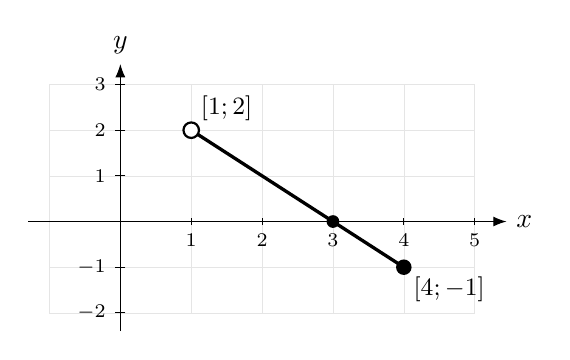
\begin{tikzpicture}[x=.90cm,y=.58cm,>=Latex]
\draw[step=1,gray!20,very thin] (-1,-2) grid (5,3);
\draw[->] (-1.3,0)--(5.45,0) node[right] {$x$};
\draw[->] (0,-2.4)--(0,3.45) node[above] {$y$};
\foreach \x in {1,2,3,4,5}{\draw (\x,.07)--(\x,-.07) node[below,font=\scriptsize] {$\x$};}
\foreach \y in {-2,-1,1,2,3}{\draw (.07,\y)--(-.07,\y) node[left,font=\scriptsize] {$\y$};}
\draw[very thick] (1,2)--(4,-1);
\draw[fill=white,thick] (1,2) circle (2.8pt);
\fill (4,-1) circle (2.8pt);
\fill (3,0) circle (2.3pt);
\node[font=\small,above right] at (1,2) {$[1;2]$};
\node[font=\small,below right] at (4,-1) {$[4;-1]$};
\end{tikzpicture}
\end{center}

\blok{Samostatné procvičení}
\begin{zadaniReseniBox}[title={Úlohy pro žáky}]
\begin{enumerate}[label=\alph*)]
\item Pro $f(x)=\tfrac12x-2$, $D(f)=\mathbb R$, určete oba průsečíky s osami.
\item Pro $g(x)=-2$ na $\langle-1;3)$ určete graf, obor hodnot a průsečík s osou $y$.
\item Pro $h(x)=2x+1$ na $\langle0;2)$ určete krajní body grafu, $H(h)$ a průsečíky s osami.
\end{enumerate}
\tcblower
\begin{enumerate}[label=\alph*)]
\item $[0;-2]$ a $[4;0]$; protože $f(4)=0$.
\item Vodorovná část přímky $y=-2$ od plného $[-1;-2]$ do prázdného $[3;-2]$;
$H(g)=\{-2\}$, průsečík s osou $y$ je $[0;-2]$.
\item Plný $[0;1]$, prázdný $[2;5]$, $H(h)=\langle1;5)$.
S osou $y$ je průsečík $[0;1]$; osa $x$ se grafu netýká,
protože nulový bod $-\tfrac12$ neleží v definičním oboru.
\end{enumerate}
\end{zadaniReseniBox}

\blok{Volitelná rezerva}
\begin{zadaniReseniBox}[title={Vodorovná a svislá přímka}]
Je množina bodů $x=2$ grafem funkce $y=f(x)$? Jak se liší od $y=2$?
\tcblower
$x=2$ je svislá přímka: jedinému argumentu $2$ by odpovídalo mnoho hodnot $y$,
proto to není graf funkce $y=f(x)$. $y=2$ je vodorovná přímka, tedy graf
konstantní funkce na $\mathbb R$.
\end{zadaniReseniBox}

\blok{Domácí úkol}
\begin{zadaniReseniBox}[title={Domácí procvičení}]
\begin{enumerate}[label=\alph*)]
\item Určete průsečíky s osami funkce $f(x)=-3x+6$ na $\mathbb R$.
\item Funkce $g(x)=4$ je zadána na $\{-2,0,3\}$. Vypište graf jako množinu bodů a určete $H(g)$.
\item Funkce $h(x)=x-2$ je zadána na $(0;3\rangle$. Určete krajní body a průsečíky s osami.
\item Je funkce $k(x)=0$ na $\mathbb R$ prostá, sudá a lichá? Zdůvodněte.
\end{enumerate}
\tcblower
\begin{enumerate}[label=\alph*)]
\item $[0;6]$ a $[2;0]$.
\item $\{[-2;4],[0;4],[3;4]\}$, $H(g)=\{4\}$; graf tvoří tři izolované body.
\item Prázdný $[0;-2]$ a plný $[3;1]$; osa $x$ v bodě $[2;0]$;
osa $y$ bez průsečíku, neboť $0$ není přípustný argument.
\item Není prostá (různé argumenty mají stejnou hodnotu). Je sudá i lichá,
protože $k(-x)=0=k(x)=-k(x)$ pro každé reálné $x$.
\end{enumerate}
\end{zadaniReseniBox}
\poznamka{Důsledně používej český zápis bodů $[x;y]$ a intervalů.
U průsečíku s osou $y$ kontroluj, zda nula opravdu patří do $D(f)$.
Hodina 66 využije konstantní funkci jako mezní hodnotu reálné veličiny.}
\end{document}
